\section[Orientation histogram detector (Triangle tracker)]{Orientation histogram detector}
\label{sec:ohd}

\subsection{Introduction}
\label{sec:ohd:intro}

    \marginpar{
        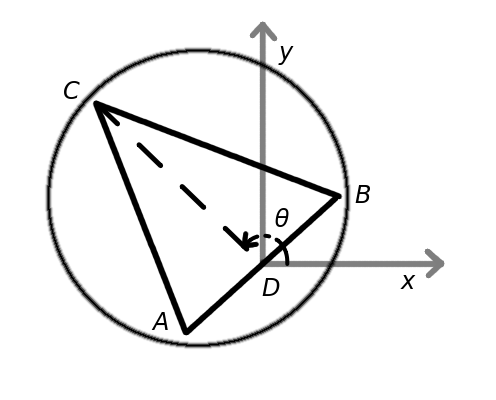
\includegraphics[width=5cm]{./img/orientation.png}
        \captionof{figure}[Calculation of the orientation]{%
        The orientation $\theta$ is the angle between the
        line $\overline{CD}$ and the $x$ axis. It ranges
        counterclockwise from 0 to 2$\pi$.}
        \label{fig:orientation}
    }

    I first built a detector to detect the robot position and orientation. 
    To do so, I used a histogram detector to detect three dots and calculate
    the angle of the height of the triangle. In order to work properly, two 
    points must be clearly closer to form a triangle that is near to be 
    isosceles.

    This detector has been split and renamed by Thomas Lampe. 
    To use a similar detector, 
    use the HistogramDetector and the 
    TriangleTracker. See the \ref{sec:ohd:edit} section for more 
    information.

\subsection{Detection of the object and his orientation}

\begin{figure}
    \caption{Detection of the position and orientation}
    \begin{subfigure}[h]{0.50\textwidth}
        \centering
        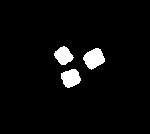
\includegraphics[width=0.80\textwidth]{./img/OrientationDetector_detect.png}
        \caption[Detection of the points]{Detection of the points --
        
        The points are detected and their size are evaluted to 
        discriminate them from noise}
        \label{fig:pointdetection}
    \end{subfigure}
    ~
    \begin{subfigure}[h]{0.50\textwidth}
        \centering
        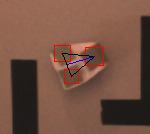
\includegraphics[width=0.80\textwidth]{./img/OrientationDetector_image.png}
        \caption[Detection of the orientation]{Detection of the 
        orientation --

        The points positions are evaluated and the orientation is 
        calculated from point C to D (see figure \ref{fig:orientation})}
        \label{fig:orientationdetection}
    \end{subfigure}
    \label{fig:podetection}
\end{figure}
 
    The detector first detects blobs with the help of the histogram 
    detector (figure \ref{fig:pointdetection}). When this is done, it 
    iterate through the blobs and selects 
    the three biggest ones.  It then selects the two closer points and 
    calculates the line from D to C to get the angle theta (figure
    \ref{fig:orientation}), which is the 
    orientation of the object (figure \ref{fig:orientationdetection}).
   \\
    \\
    The position of the object is the mean position of the three points.

\subsection{Improvements}
\label{sec:ohd:improvments}

    The detector is weak to noise. If one of the dots is not correctly 
    detected and get smaller than some noisy blobs, the noisy blob is 
    detected as one of the dots and the calculated position is not 
    good.

    We could keep the three points in memory and take the closest points 
    at the next detection. It could still be unstable if the movement is 
    fast and noise is closer than the next position. The best option might 
    be to weight the distances with the size of the blobs. 
    \\
    \\
    The detector was to unstable because of small changes in ambient light.
    Also, we needed to remove the Khepera from under the camera every time 
    we restarted the detector, because the histogram should not contain 
    colors of the Khepera. So I decided to build a new detector that would 
    detect specific colors. This way, the detector would be more reliable 
    or could me more easily reconfigured during ambient light changes. 
    Also, we could also leave the Khepera under the camera all the time. 
    \\
    \\
    \marginpar{
        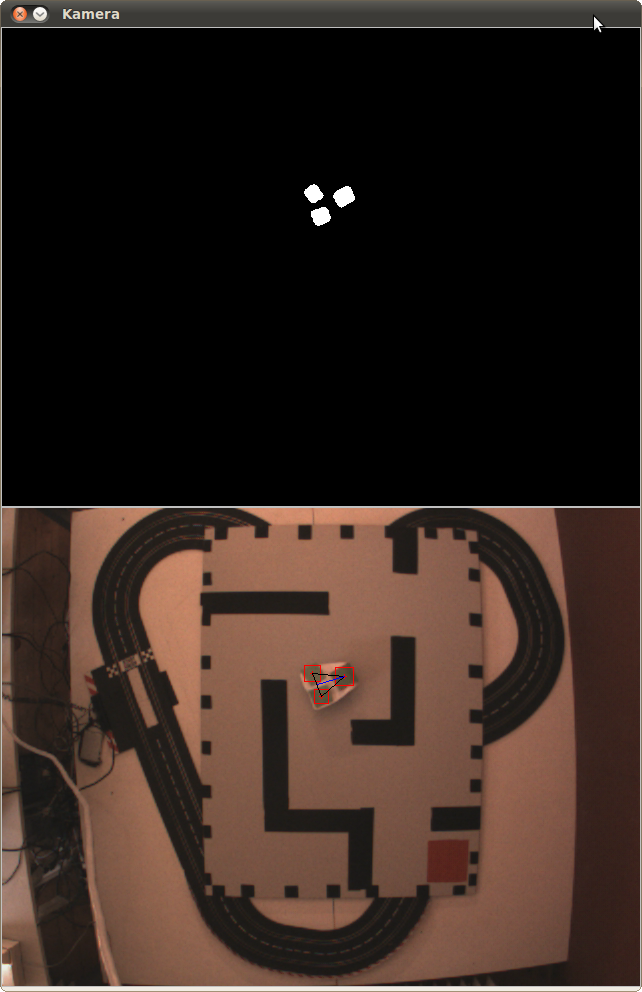
\includegraphics[width=4.5cm]{./img/OrientationDetector_full.png}
        \captionof{figure}[Interface example of the Orientation histogram
        detector]{Interface example of the Orientation histogram
        detector -- The detected points (white on black) are above and 
        the calculated 
        triangle and orientation are underneath}
    }
    The Orientation histogram detector is not included in Tapir because 
    the Orientation color detector works better on every aspects, so the 
    one is useless.

\subsection{How to use}
\label{sec:ohd:howto}
    \begin{enumerate}
        \item Find a color that is well detected with the detector 
            in the desired environment. Square of colored paper 
            seems to fare better than 
            colored dots with pencils on white paper 
        \item Put 3 dots of the found color on the object you want to 
            detect. Inclined surface reflects less strong light 
            and thus is easier to detect.
        \item Get the object out of the vision.
        \item Start the detector and wait a few second until it stops 
            adding frames to the histogram.
        \item Add the object to the environment. 
        \item It should be detector properly. If not, try modifying the 
            ambiant light or adding more frames with the ' ' (space) 
            key while the robot is removed from the view.
    \end{enumerate}

\subsubsection{Parameters for configuration file}
\label{sec:ohd:howto:params}
    \begin{description} \itemindent=-15pt
        \item[examples\_init] \hfill \\ number of frames added to the histogram at the beginning
        \item[examples\_renew] \hfill \\ number of frames added to the histogram when pressing ‘+’
        \item[box] \hfill \\ draw box around all blobs in the image
        \item[area] \hfill \\ (min,max) define minimum and maximum size to detect objects (objects smaller than min or bigger than max are not detected)
        \item[filename] \hfill \\ filename where to save histogram (optional)
        \item[autoload] \hfill \\ load the histogram saved in ‘filename’ at the beginning
    \end{description}

\subsubsection{Keys}
\label{sec:ohd:howto:keys}
    \begin{description} \itemindent=-15pt
        \item['+'] \hfill \\ add 'examples\_renew' frames to the histogram
        \item[' ' (space)] \hfill \\ add frames to the histogram until ' ' (space) his pressed again.
        \item['s'] \hfill \\ save the histogram in 'filename'
        \item['l'] \hfill \\ load the 'filename' histogram
    \end{description}

\subsection{Edit}
\label{sec:ohd:edit}
During the refactoring of the modules to make them compatible with the 
new Tapir interface, Thomas Lampe have separated the detection and blob 
selection process. He placed the selection process in a TriangleTracker, 
which makes more sense since it is a tracking process. The detector 
remains the one on which I built the orientation histogram detector; 
HistogramDetector. The major improvements to stabilise more the detection 
of the triangle will now lie in TriangleTracker rather than in 
HistogramDetector.
